\section{Einsatz von KI zur Erkennung von Thematiken}\label{sec:ai-recognition}

\subsection{Allgemeines}

Ein weiterer Teil dieses Projektes besteht darin, die von den \nameref{sec:topciModeling}-Methoden erzeugten (unbenannten) Topics zu benennen. Diese Aufgabe kann einer Künstlichen Intelligenz ohne Bedenken weitergegeben werden. Da mit dem Aufkommen neuerer und effizienterer Technologien in den vergangenen Jahren zeitgleich eine beträchtliche Anzahl von sogenannten \glspl{Foundation Model} entstanden ist, können solche für Projekte wie diesem eingesetzt werden.

\smallskip\par\noindent
Im Anschluss sollen mehrere Sprachmodelle einzeln vorgestellt und auf ihre technischen Eigenschaften sowie Systemanforderungen analysiert werden. Des Weiteren soll untersucht werden, wie diese Modelle durch Fine-Tuning für diesen projektspezifischen Anwendungsfall angepasst werden können.

\subsection{Large Language Models}

\subsubsection{Grundlegendes}

...

\subsubsection{\acrfull{ac:gpt}}\label{sec:gpt}

...

\smallskip\par\noindent
Im Gegensatz zu den anderen angeführten Modellen stehen die neueren Entwicklungen der \acrshort{ac:gpt}-Reihe nicht mehr unter einer freien Lizenz, weshalb das Interagieren mit diesen Modellen nur über eine API\footnote{\url{https://platform.openai.com/docs/guides/gpt}} und das auch nicht immer kostenlos möglich ist. Unabhängig davon lässt sich jedoch \nameref{sec:prompt_engineering} mit ihnen betreiben.

\subsubsection{Llama}\label{sec:llama}

...

\smallskip\par\noindent
Bei \acrshort{ac:llama}-V2 ist mit folgenden Speicherplatzanforderungen zu rechnen\footnote{Diese Angaben beziehen sich auf die (unveränderten) Basis-Modelle der einzelnen Varianten. Die Angaben des benötigten Speicherplatzes beziehen sich auf die Dateigrößen der auf \url{https://huggingface.co/} zum Zeitpunkt dieses Schreibens veröffentlichten Gewichte.\label{note:requirements}}\textsuperscript{,}\footnote{Eine weitere Variante, \acrshort{ac:llama}-34B, wurde ebenfalls entwickelt, aber zu diesem Zeitpunkt noch nicht veröffentlicht.}:

\begin{table}
    \centering
    \begin{tabularx}{8cm}{| >{\raggedright\arraybackslash}X | >{\raggedleft\arraybackslash}X |}
        \hline
        \textbf{Variante} & \textbf{Speicherplatz} \\
        \hline
        \acrshort{ac:llama}-7B   & 13.5 GB \\
        \hline
        \acrshort{ac:llama}-13B  & 26.0 GB \\
        \hline
        \acrshort{ac:llama}-70B & 120.4 GB \\
        \hline
    \end{tabularx}
    \caption{Anforderungen der einzelnen \acrshort{ac:llama}-Varianten}
\end{table}

\paragraph*{Trainingsdaten und Mehrsprachigkeit}\mbox{}

\smallskip\noindent
Die \acrshort{ac:llama}-Modelle wurden zu einem Großteil mit englischen Texten trainiert, andere Sprachen sind stark unterrepräsentiert:

\begin{table}
    \centering
    \begin{tabularx}{8cm}{| >{\raggedright\arraybackslash}X | >{\raggedleft\arraybackslash}X |}
        \hline
        \textbf{Sprache} &  \textbf{Anteil} \\
        \hline
        Englisch   &   89.70\% \\
        \hline
        Deutsch    &   0.17\% \\
        \hline
        Französisch&   0.16\% \\
        \hline
        Schwedisch &   0.15\% \\
        \hline
    \end{tabularx}
    \caption{Mehrsprachigkeit in den Trainingsdaten von \acrshort{ac:llama} (Ausschnitt) \cite[22]{touvron2023llama}}
    \label{tab:my_label}
\end{table}

\subsubsection{Falcon}\label{sec:falcon}

...

\par\noindent Für die einzelnen Varianten des Falcon-Sprachmodells sind folgende Anforderungen gegeben\footref{note:requirements}:

\begin{table}
    \centering
    \begin{tabularx}{12cm}{ | >{\raggedright\arraybackslash}X | >{\raggedleft\arraybackslash}X | >{\raggedleft\arraybackslash}X |}
        \hline
        \textbf{Variante} & \textbf{Speicherplatz} & \textbf{VRAM \cite{falcon}} \\
        \hline
        Falcon-7B   & 14.5 GB   & 16 GB \\
        \hline
        Falcon-40B  & 83.7 GB   & 85-100 GB \\
        \hline
        Falcon-180B & 360.0 GB  & 400 GB \\
        \hline
    \end{tabularx}
    \caption{Anforderungen der einzelnen Falcon-Varianten}
\end{table}

\paragraph*{Trainingsdaten und Mehrsprachigkeit}\mbox{}

\smallskip\noindent
Alle Falcon-Modelle wurden mit dem frei verfügbaren RefinedWeb-Datensatz\footnote{\url{https://huggingface.co/datasets/tiiuae/falcon-refinedweb}} trainiert. Für die Varianten ab Falcon-40B sind folgende Angaben bezüglich der Mehrsprachigkeit gemacht worden:

\smallskip\par\noindent
...

\subsubsection{Fazit}

...

\subsection{Anpassen von vortrainierten Modellen}

\subsubsection{Grundlegendes}

Wie oben bereits ersichtlich ist, wird zum (Vor-)Trainieren auf eine breite Masse von unterschiedlichsten textbasierten Datensätzen zurückgegriffen. Die daraus resultierenden Sprachmodelle können damit allgemein gut eingesetzt werden, für einzelne bestimmte Aufgaben schneiden sie jedoch schlechter ab. Dass diese Modelle lediglich vortrainiert werden, hat den Hintergrund, dass Entwickler damit ein Basis-Modell besitzen, welches sie für ihre eigenen Zwecke spezialisieren (\enquote{fine-tunen}) können. Nun soll untersucht werden, welche Möglichkeiten des Fine-Tunens zur Verfügung stehen und welche für dieses Projekt das gewünschte Ergebnis erzielen können.

\subsubsection{\acrfull{ac:lora}}\label{sec:lora}

...

\smallskip\par\noindent
Diese Methode zeichnet sich dadurch aus, dass die vortrainierten Gewichte eingefroren und nur bestimmte Parameter angepasst werden, was die Speicher- und Leistungsanforderungen erheblich senkt \cite[1]{Hu2021}. Gleichzeitig ist damit die Gefahr eines Qualitätsverlustes durch \gls{Catastrophic Forgetting} nicht mehr gegeben \cite{HugFaceLoRa}.

\begin{figure}
    \centering
    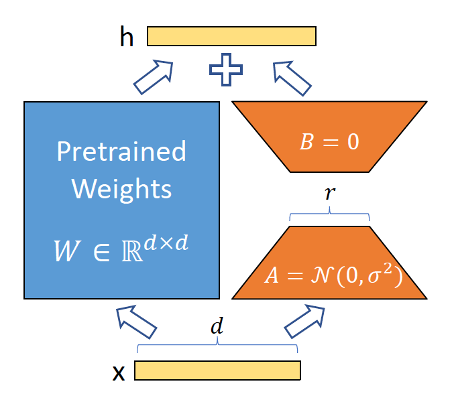
\includegraphics[scale=0.4]{images/asuender/lora.png}
    \caption{Funktionsweise von \acrshort{ac:lora}. Es werden hier nur $A$ und $B$ trainiert \cite[1]{Hu2021}.}
    \label{fig:lora}
\end{figure}

\subsubsection{Prompt Engineering}\label{sec:prompt_engineering}

...

\smallskip\par\noindent
Ein großer Nachteil ist die Tatsache, dass das Erstellen der Prompts nicht vollständig automatisiert ablaufen kann und noch menschliche Hilfe benötigt wird, um die Eingaben vor dem Weitergeben an das Modell zu überprüfen \cite[1]{Lester2021}. Des Weiteren kann die Qualität der Ergebnisse stark davon beeinflusst werden, wie viele Zeichen im Prompt ein bestimmtes Modell unterstützt. Im Allgemeinen kommt Prompt Engineering daher an die anderen Fine Tuning-Methoden nicht heran.

\smallskip\par\noindent
Ein weiteres Problem stellt die \enquote{Ergebnissicherheit} dar. Ein entscheidender Punkt bei der Auswahl der geeigneten Tuning-Methode ist die Wahrscheinlichkeit, dass die Antwort des Sprachmodells auch tatsächlich dem erwarteten Format entspricht, da diese wiederum von einer anderen Instanz weiterverarbeitet werden muss. Es besteht hier nach wie vor eine (höhere) Gefahr, dass das Modell trotz ausreichender Instruktion nicht die gewünschten Daten liefert.

\subsubsection{Prompt Tuning}\label{sec:prompt_tuning}

...

\begin{figure}
    \centering
    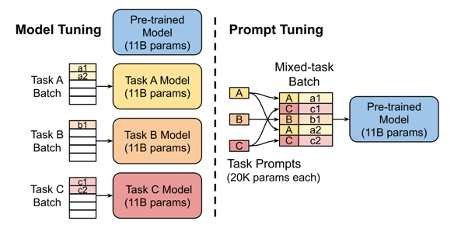
\includegraphics[scale=0.6]{images/asuender/prompt_tuning.png}
    \caption{Funktionsweise des Prompt-Tunings \cite[2]{Lester2021}}
    \label{fig:prompt_tuning}
\end{figure}

\subsubsection{Fazit}

...

\subsection{Aufbereiten von Sprachmodellen}

\subsubsection{Quantization}\label{sec:quantization}

Neben den meist sehr hohen Leitungsanforderungen stehen fortgeschrittene Sprachmodelle noch vor dem Problem des hohen Speicherbedarfs. Etwa benötigt das im Jahr 2020 veröffentlichte Modell GPT-3 unter gewissen Bedingungen 326 GB an Speicherplatz \cite[1]{Frantar2022}.

\smallskip\par\noindent
Die Hauptursache dafür sind die in den Modellen hinterlegten Parameter, die mit einer gewissen Genauigkeit als Gleitkommazahlen gespeichert werden. Typischerweise werden Sprachmodelle mit einer Genauigkeit von 32 Bits gespeichert und veröffentlicht, was die Anforderungen zum Betreiben dieser Modelle entsprechend stark erhöht. \textit{Quantization} ermöglicht es, die gespeicherten Parameter auf eine niedrigere Genauigkeit komprimieren, um sowohl die Leistungs- als auch Speicherplatzanforderungen zu senken.

\smallskip\par\noindent
Ein großer Vorteil ist, dass mit dieser harschen Anpassung der Parameter nicht zwingend ein ebenso großer Genauigkeitsverlust einhergeht. Beispielsweise soll es mit der \textbf{Q-BERT}-Methode möglich sein, bestimmte Gewichte bis auf zwei Nachkommastellen \enquote{abzuschneiden}, ohne dabei einen maximalen Genauigkeitsverlust von 2.3\% zu überschreiten \cite[1]{Shen2019}. Damit soll (theoretisch) eine bis zu 13-fache Kompression der Modellparameter erzielt werden können. Eine weitere Methode, \textbf{GPTQ}, erlaubt das schnelle Komprimieren auf eine Genauigkeit von 3 bzw. 4 Bits \cite[1]{Frantar2022}; eine entsprechende (vorläufige) Implementierung ist für Python bereits verfügbar\footnote{\url{https://github.com/PanQiWei/AutoGPTQ}}. Von den oben angeführten Modellen wird aktuell nur \nameref{sec:llama} unterstützt.

\subsection{Bereitstellen von Sprachmodellen}

\subsubsection{Text Generation Inference}

...

\subsubsection{vLLM}